% Options for packages loaded elsewhere
\PassOptionsToPackage{unicode}{hyperref}
\PassOptionsToPackage{hyphens}{url}
%
\documentclass[
]{article}
\usepackage{amsmath,amssymb}
\usepackage{lmodern}
\usepackage{iftex}
\ifPDFTeX
  \usepackage[T1]{fontenc}
  \usepackage[utf8]{inputenc}
  \usepackage{textcomp} % provide euro and other symbols
\else % if luatex or xetex
  \usepackage{unicode-math}
  \defaultfontfeatures{Scale=MatchLowercase}
  \defaultfontfeatures[\rmfamily]{Ligatures=TeX,Scale=1}
\fi
% Use upquote if available, for straight quotes in verbatim environments
\IfFileExists{upquote.sty}{\usepackage{upquote}}{}
\IfFileExists{microtype.sty}{% use microtype if available
  \usepackage[]{microtype}
  \UseMicrotypeSet[protrusion]{basicmath} % disable protrusion for tt fonts
}{}
\makeatletter
\@ifundefined{KOMAClassName}{% if non-KOMA class
  \IfFileExists{parskip.sty}{%
    \usepackage{parskip}
  }{% else
    \setlength{\parindent}{0pt}
    \setlength{\parskip}{6pt plus 2pt minus 1pt}}
}{% if KOMA class
  \KOMAoptions{parskip=half}}
\makeatother
\usepackage{xcolor}
\usepackage[margin=1in]{geometry}
\usepackage{color}
\usepackage{fancyvrb}
\newcommand{\VerbBar}{|}
\newcommand{\VERB}{\Verb[commandchars=\\\{\}]}
\DefineVerbatimEnvironment{Highlighting}{Verbatim}{commandchars=\\\{\}}
% Add ',fontsize=\small' for more characters per line
\usepackage{framed}
\definecolor{shadecolor}{RGB}{248,248,248}
\newenvironment{Shaded}{\begin{snugshade}}{\end{snugshade}}
\newcommand{\AlertTok}[1]{\textcolor[rgb]{0.94,0.16,0.16}{#1}}
\newcommand{\AnnotationTok}[1]{\textcolor[rgb]{0.56,0.35,0.01}{\textbf{\textit{#1}}}}
\newcommand{\AttributeTok}[1]{\textcolor[rgb]{0.77,0.63,0.00}{#1}}
\newcommand{\BaseNTok}[1]{\textcolor[rgb]{0.00,0.00,0.81}{#1}}
\newcommand{\BuiltInTok}[1]{#1}
\newcommand{\CharTok}[1]{\textcolor[rgb]{0.31,0.60,0.02}{#1}}
\newcommand{\CommentTok}[1]{\textcolor[rgb]{0.56,0.35,0.01}{\textit{#1}}}
\newcommand{\CommentVarTok}[1]{\textcolor[rgb]{0.56,0.35,0.01}{\textbf{\textit{#1}}}}
\newcommand{\ConstantTok}[1]{\textcolor[rgb]{0.00,0.00,0.00}{#1}}
\newcommand{\ControlFlowTok}[1]{\textcolor[rgb]{0.13,0.29,0.53}{\textbf{#1}}}
\newcommand{\DataTypeTok}[1]{\textcolor[rgb]{0.13,0.29,0.53}{#1}}
\newcommand{\DecValTok}[1]{\textcolor[rgb]{0.00,0.00,0.81}{#1}}
\newcommand{\DocumentationTok}[1]{\textcolor[rgb]{0.56,0.35,0.01}{\textbf{\textit{#1}}}}
\newcommand{\ErrorTok}[1]{\textcolor[rgb]{0.64,0.00,0.00}{\textbf{#1}}}
\newcommand{\ExtensionTok}[1]{#1}
\newcommand{\FloatTok}[1]{\textcolor[rgb]{0.00,0.00,0.81}{#1}}
\newcommand{\FunctionTok}[1]{\textcolor[rgb]{0.00,0.00,0.00}{#1}}
\newcommand{\ImportTok}[1]{#1}
\newcommand{\InformationTok}[1]{\textcolor[rgb]{0.56,0.35,0.01}{\textbf{\textit{#1}}}}
\newcommand{\KeywordTok}[1]{\textcolor[rgb]{0.13,0.29,0.53}{\textbf{#1}}}
\newcommand{\NormalTok}[1]{#1}
\newcommand{\OperatorTok}[1]{\textcolor[rgb]{0.81,0.36,0.00}{\textbf{#1}}}
\newcommand{\OtherTok}[1]{\textcolor[rgb]{0.56,0.35,0.01}{#1}}
\newcommand{\PreprocessorTok}[1]{\textcolor[rgb]{0.56,0.35,0.01}{\textit{#1}}}
\newcommand{\RegionMarkerTok}[1]{#1}
\newcommand{\SpecialCharTok}[1]{\textcolor[rgb]{0.00,0.00,0.00}{#1}}
\newcommand{\SpecialStringTok}[1]{\textcolor[rgb]{0.31,0.60,0.02}{#1}}
\newcommand{\StringTok}[1]{\textcolor[rgb]{0.31,0.60,0.02}{#1}}
\newcommand{\VariableTok}[1]{\textcolor[rgb]{0.00,0.00,0.00}{#1}}
\newcommand{\VerbatimStringTok}[1]{\textcolor[rgb]{0.31,0.60,0.02}{#1}}
\newcommand{\WarningTok}[1]{\textcolor[rgb]{0.56,0.35,0.01}{\textbf{\textit{#1}}}}
\usepackage{graphicx}
\makeatletter
\def\maxwidth{\ifdim\Gin@nat@width>\linewidth\linewidth\else\Gin@nat@width\fi}
\def\maxheight{\ifdim\Gin@nat@height>\textheight\textheight\else\Gin@nat@height\fi}
\makeatother
% Scale images if necessary, so that they will not overflow the page
% margins by default, and it is still possible to overwrite the defaults
% using explicit options in \includegraphics[width, height, ...]{}
\setkeys{Gin}{width=\maxwidth,height=\maxheight,keepaspectratio}
% Set default figure placement to htbp
\makeatletter
\def\fps@figure{htbp}
\makeatother
\setlength{\emergencystretch}{3em} % prevent overfull lines
\providecommand{\tightlist}{%
  \setlength{\itemsep}{0pt}\setlength{\parskip}{0pt}}
\setcounter{secnumdepth}{-\maxdimen} % remove section numbering
\usepackage{booktabs}
\usepackage{longtable}
\usepackage{array}
\usepackage{multirow}
\usepackage{wrapfig}
\usepackage{float}
\usepackage{colortbl}
\usepackage{pdflscape}
\usepackage{tabu}
\usepackage{threeparttable}
\usepackage{threeparttablex}
\usepackage[normalem]{ulem}
\usepackage{makecell}
\usepackage{xcolor}
\ifLuaTeX
  \usepackage{selnolig}  % disable illegal ligatures
\fi
\IfFileExists{bookmark.sty}{\usepackage{bookmark}}{\usepackage{hyperref}}
\IfFileExists{xurl.sty}{\usepackage{xurl}}{} % add URL line breaks if available
\urlstyle{same} % disable monospaced font for URLs
\hypersetup{
  pdftitle={analy\_theta},
  pdfauthor={Haodong Li},
  hidelinks,
  pdfcreator={LaTeX via pandoc}}

\title{analy\_theta}
\author{Haodong Li}
\date{2022-11-28}

\begin{document}
\maketitle

\hypertarget{experiment-and-question}{%
\subsection{1. Experiment and question}\label{experiment-and-question}}

The LEADER trial is a multi-centre randomised trial to determine
Liraglutide (GLP-1) effects on cardiovascular events. So the original
treatment variable is Liraglutide/Placebo and outcome consists of
several cardiovascular events. It is known that GLP-1 users are also
often on statins and other cardiovascular drugs. In this project, we
want to explore the heterogeneity of liraglutide treatment effect among
concomitant medication (especially statin) users, with diabetes
progression as primary outcome, cardiovascular events as second outcome.

\hypertarget{overview-of-data}{%
\subsection{2. Overview of data}\label{overview-of-data}}

\begin{Shaded}
\begin{Highlighting}[]
\NormalTok{outcome }\OtherTok{=} \StringTok{\textquotesingle{}diab\textquotesingle{}}\NormalTok{; t }\OtherTok{=} \DecValTok{24}
\NormalTok{df }\OtherTok{\textless{}{-}} \FunctionTok{get\_data}\NormalTok{(outcome, t)}

\NormalTok{nodes }\OtherTok{\textless{}{-}} \FunctionTok{list}\NormalTok{(}\AttributeTok{W =} \FunctionTok{setdiff}\NormalTok{(}\FunctionTok{names}\NormalTok{(df), }\FunctionTok{c}\NormalTok{(}\StringTok{"Y"}\NormalTok{, }\StringTok{"A"}\NormalTok{)),}
              \AttributeTok{A =} \StringTok{\textquotesingle{}A\textquotesingle{}}\NormalTok{,}
              \AttributeTok{Y =} \StringTok{\textquotesingle{}Y\textquotesingle{}}\NormalTok{)}

\NormalTok{p\_before }\OtherTok{=} \FunctionTok{ncol}\NormalTok{(df)}\SpecialCharTok{{-}}\DecValTok{2}
\NormalTok{df }\OtherTok{\textless{}{-}} \FunctionTok{process\_missing}\NormalTok{(df, nodes)}\SpecialCharTok{$}\NormalTok{data}
\FunctionTok{print}\NormalTok{(}\FunctionTok{paste0}\NormalTok{(}\StringTok{"data dimension (before): n="}\NormalTok{, }\FunctionTok{nrow}\NormalTok{(df), }\StringTok{", p="}\NormalTok{, p\_before))}
\end{Highlighting}
\end{Shaded}

\begin{verbatim}
## [1] "data dimension (before): n=4169, p=51"
\end{verbatim}

\begin{Shaded}
\begin{Highlighting}[]
\FunctionTok{print}\NormalTok{(}\FunctionTok{paste0}\NormalTok{(}\StringTok{"data dimension (after): n="}\NormalTok{, }\FunctionTok{nrow}\NormalTok{(df), }\StringTok{", p="}\NormalTok{, }\FunctionTok{ncol}\NormalTok{(df)}\SpecialCharTok{{-}}\DecValTok{2}\NormalTok{))}
\end{Highlighting}
\end{Shaded}

\begin{verbatim}
## [1] "data dimension (after): n=4169, p=61"
\end{verbatim}

\begin{Shaded}
\begin{Highlighting}[]
\CommentTok{\# Table of Baseline Characteristics }
\NormalTok{df\_w\_summary }\OtherTok{\textless{}{-}}\NormalTok{ df\_w }\SpecialCharTok{\%\textgreater{}\%} 
  \FunctionTok{filter}\NormalTok{(INSNVFL }\SpecialCharTok{==} \ConstantTok{FALSE}\NormalTok{) }\SpecialCharTok{\%\textgreater{}\%} 
  \FunctionTok{select}\NormalTok{(}\SpecialCharTok{{-}}\FunctionTok{c}\NormalTok{(}\StringTok{"USUBJID"}\NormalTok{, }\StringTok{"INSNVFL"}\NormalTok{)) }\SpecialCharTok{\%\textgreater{}\%} 
  \FunctionTok{mutate}\NormalTok{(}\AttributeTok{A =} \FunctionTok{ifelse}\NormalTok{(A }\SpecialCharTok{==} \DecValTok{1}\NormalTok{, }\StringTok{"Liraglutide"}\NormalTok{, }\StringTok{"Placebo"}\NormalTok{))}

\NormalTok{df\_w\_summary }\OtherTok{\textless{}{-}}\NormalTok{ labelled}\SpecialCharTok{::}\FunctionTok{remove\_labels}\NormalTok{(df\_w\_summary)}
\NormalTok{tbl }\OtherTok{\textless{}{-}} \FunctionTok{table1}\NormalTok{(}\SpecialCharTok{\textasciitilde{}}\NormalTok{. }\SpecialCharTok{|}\NormalTok{ A, }\AttributeTok{data =}\NormalTok{ df\_w\_summary, }\AttributeTok{caption =} \StringTok{"Baseline characteristics in LEADER"}\NormalTok{)}
\CommentTok{\# kable(as.data.frame(tbl), longtable=TRUE, booktabs=TRUE) }
\end{Highlighting}
\end{Shaded}

\newpage

\begin{Shaded}
\begin{Highlighting}[]
\NormalTok{tbl }\SpecialCharTok{\%\textgreater{}\%} \FunctionTok{t1kable}\NormalTok{(}\AttributeTok{longtable=}\ConstantTok{TRUE}\NormalTok{) }\SpecialCharTok{\%\textgreater{}\%}
  \FunctionTok{kable\_styling}\NormalTok{(., }\AttributeTok{font\_size =} \DecValTok{9}\NormalTok{, }\AttributeTok{latex\_options =} \StringTok{"hold\_position"}\NormalTok{, }\AttributeTok{position =} \StringTok{"center"}\NormalTok{)}
\end{Highlighting}
\end{Shaded}

\begingroup\fontsize{9}{11}\selectfont

\begin{longtable}[t]{llll}
\caption{\label{tab:unnamed-chunk-4}Baseline characteristics in LEADER}\\
\toprule
  & Liraglutide & Placebo & Overall\\
\midrule
 & (N=2038) & (N=2131) & (N=4169)\\
\addlinespace[0.3em]
\multicolumn{4}{l}{\textbf{AGE}}\\
\hspace{1em}Mean (SD) & 64.5 (7.22) & 64.5 (7.13) & 64.5 (7.17)\\
\hspace{1em}Median [Min, Max] & 64.0 [50.0, 87.0] & 64.0 [50.0, 88.0] & 64.0 [50.0, 88.0]\\
\hspace{1em}Missing & 1 (0.0\%) & 0 (0\%) & 1 (0.0\%)\\
\addlinespace[0.3em]
\multicolumn{4}{l}{\textbf{SEX}}\\
\hspace{1em}F & 764 (37.5\%) & 829 (38.9\%) & 1593 (38.2\%)\\
\hspace{1em}M & 1274 (62.5\%) & 1302 (61.1\%) & 2576 (61.8\%)\\
\addlinespace[0.3em]
\multicolumn{4}{l}{\textbf{RACE}}\\
\hspace{1em}ASIAN & 199 (9.8\%) & 210 (9.9\%) & 409 (9.8\%)\\
\hspace{1em}BLACK & 185 (9.1\%) & 223 (10.5\%) & 408 (9.8\%)\\
\hspace{1em}OTHER & 89 (4.4\%) & 76 (3.6\%) & 165 (4.0\%)\\
\hspace{1em}WHITE & 1565 (76.8\%) & 1622 (76.1\%) & 3187 (76.4\%)\\
\addlinespace[0.3em]
\multicolumn{4}{l}{\textbf{COUNTRY}}\\
\hspace{1em}Africa & 64 (3.1\%) & 86 (4.0\%) & 150 (3.6\%)\\
\hspace{1em}America & 956 (46.9\%) & 1011 (47.4\%) & 1967 (47.2\%)\\
\hspace{1em}Asia & 337 (16.5\%) & 330 (15.5\%) & 667 (16.0\%)\\
\hspace{1em}Europe & 615 (30.2\%) & 644 (30.2\%) & 1259 (30.2\%)\\
\hspace{1em}Pacific & 66 (3.2\%) & 60 (2.8\%) & 126 (3.0\%)\\
\addlinespace[0.3em]
\multicolumn{4}{l}{\textbf{SMOKER}}\\
\hspace{1em}CURRENT SMOKER & 236 (11.6\%) & 246 (11.5\%) & 482 (11.6\%)\\
\hspace{1em}NEVER SMOKED & 853 (41.9\%) & 886 (41.6\%) & 1739 (41.7\%)\\
\hspace{1em}PREVIOUS SMOKER & 949 (46.6\%) & 999 (46.9\%) & 1948 (46.7\%)\\
\addlinespace[0.3em]
\multicolumn{4}{l}{\textbf{NYHACLAS}}\\
\hspace{1em}NYHA CLAS NA & 1672 (82.0\%) & 1760 (82.6\%) & 3432 (82.3\%)\\
\hspace{1em}NYHA CLASS I & 75 (3.7\%) & 78 (3.7\%) & 153 (3.7\%)\\
\hspace{1em}NYHA CLASS II & 244 (12.0\%) & 244 (11.5\%) & 488 (11.7\%)\\
\hspace{1em}NYHA CLASS III & 47 (2.3\%) & 49 (2.3\%) & 96 (2.3\%)\\
\addlinespace[0.3em]
\multicolumn{4}{l}{\textbf{DIABDUR}}\\
\hspace{1em}Mean (SD) & 15.5 (7.91) & 15.3 (8.01) & 15.4 (7.96)\\
\hspace{1em}Median [Min, Max] & 14.2 [0.100, 54.9] & 14.3 [0.100, 61.0] & 14.3 [0.100, 61.0]\\
\hspace{1em}Missing & 4 (0.2\%) & 3 (0.1\%) & 7 \vphantom{1} (0.2\%)\\
\addlinespace[0.3em]
\multicolumn{4}{l}{\textbf{ANTDBFL}}\\
\hspace{1em}Insulin-OAD & 361 (17.7\%) & 377 (17.7\%) & 738 (17.7\%)\\
\hspace{1em}Insulin+OAD(s) & 1677 (82.3\%) & 1754 (82.3\%) & 3431 (82.3\%)\\
\addlinespace[0.3em]
\multicolumn{4}{l}{\textbf{AHYPERFL}}\\
\hspace{1em}Yes & 192 (9.4\%) & 189 (8.9\%) & 381 (9.1\%)\\
\hspace{1em}No & 1846 (90.6\%) & 1942 (91.1\%) & 3788 (90.9\%)\\
\addlinespace[0.3em]
\multicolumn{4}{l}{\textbf{INCPASSN}}\\
\hspace{1em}Mean (SD) & 5.00 (0.0585) & 4.99 (0.0717) & 5.00 (0.0656)\\
\hspace{1em}Median [Min, Max] & 5.00 [4.00, 5.00] & 5.00 [4.00, 5.00] & 5.00 [4.00, 5.00]\\
\addlinespace[0.3em]
\multicolumn{4}{l}{\textbf{BMIBL}}\\
\hspace{1em}Mean (SD) & 32.8 (6.18) & 33.0 (6.47) & 32.9 (6.33)\\
\hspace{1em}Median [Min, Max] & 32.0 [19.7, 66.5] & 32.0 [18.0, 81.0] & 32.0 [18.0, 81.0]\\
\hspace{1em}Missing & 3 (0.1\%) & 2 (0.1\%) & 5 (0.1\%)\\
\addlinespace[0.3em]
\multicolumn{4}{l}{\textbf{PULSEBL}}\\
\hspace{1em}Mean (SD) & 72.8 (11.3) & 72.8 (11.6) & 72.8 (11.4)\\
\hspace{1em}Median [Min, Max] & 72.0 [37.0, 172] & 72.0 [35.0, 121] & 72.0 [35.0, 172]\\
\addlinespace[0.3em]
\multicolumn{4}{l}{\textbf{SYSBPBL}}\\
\hspace{1em}Mean (SD) & 136 (18.7) & 136 (17.9) & 136 (18.3)\\
\hspace{1em}Median [Min, Max] & 135 [74.0, 222] & 135 [72.5, 227] & 135 [72.5, 227]\\
\addlinespace[0.3em]
\multicolumn{4}{l}{\textbf{DIABPBL}}\\
\hspace{1em}Mean (SD) & 76.1 (10.4) & 76.0 (10.3) & 76.1 (10.3)\\
\hspace{1em}Median [Min, Max] & 76.5 [43.5, 128] & 76.5 [38.5, 123] & 76.5 [38.5, 128]\\
\addlinespace[0.3em]
\multicolumn{4}{l}{\textbf{HBA1CBL}}\\
\hspace{1em}Mean (SD) & 8.93 (1.61) & 8.84 (1.52) & 8.88 (1.56)\\
\hspace{1em}Median [Min, Max] & 8.50 [5.10, 18.5] & 8.50 [5.80, 16.7] & 8.50 [5.10, 18.5]\\
\addlinespace[0.3em]
\multicolumn{4}{l}{\textbf{HDL1BL}}\\
\hspace{1em}Mean (SD) & 1.17 (0.322) & 1.16 (0.314) & 1.17 (0.318)\\
\hspace{1em}Median [Min, Max] & 1.13 [0.270, 3.21] & 1.11 [0.0800, 3.32] & 1.11 [0.0800, 3.32]\\
\hspace{1em}Missing & 40 (2.0\%) & 33 (1.5\%) & 73 \vphantom{5} (1.8\%)\\
\addlinespace[0.3em]
\multicolumn{4}{l}{\textbf{LDL1BL}}\\
\hspace{1em}Mean (SD) & 2.29 (0.915) & 2.30 (0.935) & 2.30 (0.925)\\
\hspace{1em}Median [Min, Max] & 2.12 [0.360, 8.23] & 2.14 [0.200, 7.93] & 2.12 [0.200, 8.23]\\
\hspace{1em}Missing & 40 (2.0\%) & 33 (1.5\%) & 73 \vphantom{4} (1.8\%)\\
\addlinespace[0.3em]
\multicolumn{4}{l}{\textbf{CHOL1BL}}\\
\hspace{1em}Mean (SD) & 4.35 (1.11) & 4.35 (1.15) & 4.35 (1.13)\\
\hspace{1em}Median [Min, Max] & 4.17 [1.86, 9.35] & 4.17 [1.81, 12.6] & 4.17 [1.81, 12.6]\\
\hspace{1em}Missing & 40 (2.0\%) & 33 (1.5\%) & 73 \vphantom{3} (1.8\%)\\
\addlinespace[0.3em]
\multicolumn{4}{l}{\textbf{RC}}\\
\hspace{1em}Mean (SD) & 0.883 (0.507) & 0.882 (0.565) & 0.883 (0.538)\\
\hspace{1em}Median [Min, Max] & 0.750 [-0.910, 4.87] & 0.750 [0.150, 11.0] & 0.750 [-0.910, 11.0]\\
\hspace{1em}Missing & 40 (2.0\%) & 33 (1.5\%) & 73 \vphantom{2} (1.8\%)\\
\addlinespace[0.3em]
\multicolumn{4}{l}{\textbf{RCoverHDL}}\\
\hspace{1em}Mean (SD) & 0.864 (0.717) & 0.868 (0.800) & 0.866 (0.760)\\
\hspace{1em}Median [Min, Max] & 0.669 [-0.820, 10.0] & 0.663 [0.0753, 14.7] & 0.667 [-0.820, 14.7]\\
\hspace{1em}Missing & 40 (2.0\%) & 33 (1.5\%) & 73 \vphantom{1} (1.8\%)\\
\addlinespace[0.3em]
\multicolumn{4}{l}{\textbf{TRIG1BL}}\\
\hspace{1em}Mean (SD) & 2.03 (1.36) & 2.03 (1.65) & 2.03 (1.52)\\
\hspace{1em}Median [Min, Max] & 1.66 [0.440, 13.3] & 1.65 [0.360, 36.1] & 1.65 [0.360, 36.1]\\
\hspace{1em}Missing & 40 (2.0\%) & 33 (1.5\%) & 73 (1.8\%)\\
\addlinespace[0.3em]
\multicolumn{4}{l}{\textbf{CREATBL}}\\
\hspace{1em}Mean (SD) & 92.0 (43.7) & 91.1 (43.3) & 91.5 (43.5)\\
\hspace{1em}Median [Min, Max] & 81.5 [33.0, 609] & 81.0 [20.0, 726] & 81.0 [20.0, 726]\\
\addlinespace[0.3em]
\multicolumn{4}{l}{\textbf{EGFMDRBC}}\\
\hspace{1em}Mean (SD) & 77.0 (27.8) & 77.7 (28.4) & 77.4 (28.1)\\
\hspace{1em}Median [Min, Max] & 76.2 [7.30, 200] & 77.0 [6.80, 419] & 76.5 [6.80, 419]\\
\addlinespace[0.3em]
\multicolumn{4}{l}{\textbf{RETINSEV}}\\
\hspace{1em}no retinopathy & 32 (1.6\%) & 41 (1.9\%) & 73 (1.8\%)\\
\hspace{1em}non-proliferative & 435 (21.3\%) & 397 (18.6\%) & 832 (20.0\%)\\
\hspace{1em}proliferative & 154 (7.6\%) & 162 (7.6\%) & 316 (7.6\%)\\
\hspace{1em}retinsev NA & 1417 (69.5\%) & 1531 (71.8\%) & 2948 (70.7\%)\\
\addlinespace[0.3em]
\multicolumn{4}{l}{\textbf{GERDBLFL}}\\
\hspace{1em}Yes & 943 (46.3\%) & 910 (42.7\%) & 1853 (44.4\%)\\
\hspace{1em}No & 1095 (53.7\%) & 1221 (57.3\%) & 2316 (55.6\%)\\
\addlinespace[0.3em]
\multicolumn{4}{l}{\textbf{PPIFL}}\\
\hspace{1em}Yes & 475 (23.3\%) & 495 (23.2\%) & 970 (23.3\%)\\
\hspace{1em}No & 1563 (76.7\%) & 1636 (76.8\%) & 3199 (76.7\%)\\
\addlinespace[0.3em]
\multicolumn{4}{l}{\textbf{H2BLFL}}\\
\hspace{1em}Yes & 83 (4.1\%) & 75 (3.5\%) & 158 (3.8\%)\\
\hspace{1em}No & 1955 (95.9\%) & 2056 (96.5\%) & 4011 (96.2\%)\\
\addlinespace[0.3em]
\multicolumn{4}{l}{\textbf{MIFL}}\\
\hspace{1em}Yes & 652 (32.0\%) & 658 (30.9\%) & 1310 (31.4\%)\\
\hspace{1em}No & 1386 (68.0\%) & 1473 (69.1\%) & 2859 (68.6\%)\\
\addlinespace[0.3em]
\multicolumn{4}{l}{\textbf{STROKEFL}}\\
\hspace{1em}Yes & 345 (16.9\%) & 370 (17.4\%) & 715 (17.2\%)\\
\hspace{1em}No & 1693 (83.1\%) & 1761 (82.6\%) & 3454 (82.8\%)\\
\addlinespace[0.3em]
\multicolumn{4}{l}{\textbf{REVASFL}}\\
\hspace{1em}Yes & 822 (40.3\%) & 900 (42.2\%) & 1722 (41.3\%)\\
\hspace{1em}No & 1216 (59.7\%) & 1231 (57.8\%) & 2447 (58.7\%)\\
\addlinespace[0.3em]
\multicolumn{4}{l}{\textbf{STENFL}}\\
\hspace{1em}Yes & 539 (26.4\%) & 546 (25.6\%) & 1085 (26.0\%)\\
\hspace{1em}No & 1499 (73.6\%) & 1585 (74.4\%) & 3084 (74.0\%)\\
\addlinespace[0.3em]
\multicolumn{4}{l}{\textbf{CHDFL}}\\
\hspace{1em}Yes & 182 (8.9\%) & 192 (9.0\%) & 374 (9.0\%)\\
\hspace{1em}No & 1856 (91.1\%) & 1939 (91.0\%) & 3795 (91.0\%)\\
\addlinespace[0.3em]
\multicolumn{4}{l}{\textbf{IHDFL}}\\
\hspace{1em}Yes & 522 (25.6\%) & 550 (25.8\%) & 1072 (25.7\%)\\
\hspace{1em}No & 1516 (74.4\%) & 1581 (74.2\%) & 3097 (74.3\%)\\
\addlinespace[0.3em]
\multicolumn{4}{l}{\textbf{CHFFL}}\\
\hspace{1em}Yes & 291 (14.3\%) & 293 (13.7\%) & 584 (14.0\%)\\
\hspace{1em}No & 1747 (85.7\%) & 1838 (86.3\%) & 3585 (86.0\%)\\
\addlinespace[0.3em]
\multicolumn{4}{l}{\textbf{KIDFL}}\\
\hspace{1em}Yes & 627 (30.8\%) & 623 (29.2\%) & 1250 (30.0\%)\\
\hspace{1em}No & 1411 (69.2\%) & 1508 (70.8\%) & 2919 (70.0\%)\\
\addlinespace[0.3em]
\multicolumn{4}{l}{\textbf{MICFL}}\\
\hspace{1em}Yes & 563 (27.6\%) & 619 (29.0\%) & 1182 (28.4\%)\\
\hspace{1em}No & 1475 (72.4\%) & 1512 (71.0\%) & 2987 (71.6\%)\\
\addlinespace[0.3em]
\multicolumn{4}{l}{\textbf{HYPFL}}\\
\hspace{1em}Yes & 488 (23.9\%) & 515 (24.2\%) & 1003 (24.1\%)\\
\hspace{1em}No & 1550 (76.1\%) & 1616 (75.8\%) & 3166 (75.9\%)\\
\addlinespace[0.3em]
\multicolumn{4}{l}{\textbf{LVSDFL}}\\
\hspace{1em}Yes & 472 (23.2\%) & 495 (23.2\%) & 967 (23.2\%)\\
\hspace{1em}No & 1566 (76.8\%) & 1636 (76.8\%) & 3202 (76.8\%)\\
\addlinespace[0.3em]
\multicolumn{4}{l}{\textbf{PADFL}}\\
\hspace{1em}Yes & 274 (13.4\%) & 300 (14.1\%) & 574 (13.8\%)\\
\hspace{1em}No & 1764 (86.6\%) & 1831 (85.9\%) & 3595 (86.2\%)\\
\addlinespace[0.3em]
\multicolumn{4}{l}{\textbf{CVRISK}}\\
\hspace{1em}High & 1717 (84.2\%) & 1762 (82.7\%) & 3479 (83.4\%)\\
\hspace{1em}Medium & 321 (15.8\%) & 369 (17.3\%) & 690 (16.6\%)\\
\addlinespace[0.3em]
\multicolumn{4}{l}{\textbf{HBA1CGRN}}\\
\hspace{1em}Mean (SD) & 1.56 (0.497) & 1.55 (0.498) & 1.55 (0.497)\\
\hspace{1em}Median [Min, Max] & 2.00 [1.00, 2.00] & 2.00 [1.00, 2.00] & 2.00 [1.00, \vphantom{1} 2.00]\\
\addlinespace[0.3em]
\multicolumn{4}{l}{\textbf{DDURGRN}}\\
\hspace{1em}Mean (SD) & 1.68 (0.467) & 1.66 (0.472) & 1.67 (0.470)\\
\hspace{1em}Median [Min, Max] & 2.00 [1.00, 2.00] & 2.00 [1.00, 2.00] & 2.00 [1.00, 2.00]\\
\hspace{1em}Missing & 4 (0.2\%) & 3 (0.1\%) & 7 (0.2\%)\\
\addlinespace[0.3em]
\multicolumn{4}{l}{\textbf{statin\_use}}\\
\hspace{1em}Yes & 1558 (76.4\%) & 1591 (74.7\%) & 3149 (75.5\%)\\
\hspace{1em}No & 480 (23.6\%) & 540 (25.3\%) & 1020 (24.5\%)\\
\addlinespace[0.3em]
\multicolumn{4}{l}{\textbf{antihypertensives}}\\
\hspace{1em}Yes & 1693 (83.1\%) & 1751 (82.2\%) & 3444 (82.6\%)\\
\hspace{1em}No & 345 (16.9\%) & 380 (17.8\%) & 725 (17.4\%)\\
\addlinespace[0.3em]
\multicolumn{4}{l}{\textbf{betab}}\\
\hspace{1em}Yes & 1186 (58.2\%) & 1219 (57.2\%) & 2405 (57.7\%)\\
\hspace{1em}No & 852 (41.8\%) & 912 (42.8\%) & 1764 (42.3\%)\\
\addlinespace[0.3em]
\multicolumn{4}{l}{\textbf{minera}}\\
\hspace{1em}Yes & 135 (6.6\%) & 141 (6.6\%) & 276 (6.6\%)\\
\hspace{1em}No & 1903 (93.4\%) & 1990 (93.4\%) & 3893 (93.4\%)\\
\addlinespace[0.3em]
\multicolumn{4}{l}{\textbf{adp}}\\
\hspace{1em}Yes & 1511 (74.1\%) & 1567 (73.5\%) & 3078 (73.8\%)\\
\hspace{1em}No & 527 (25.9\%) & 564 (26.5\%) & 1091 (26.2\%)\\
\addlinespace[0.3em]
\multicolumn{4}{l}{\textbf{vkantag}}\\
\hspace{1em}Yes & 135 (6.6\%) & 137 (6.4\%) & 272 (6.5\%)\\
\hspace{1em}No & 1903 (93.4\%) & 1994 (93.6\%) & 3897 (93.5\%)\\
\addlinespace[0.3em]
\multicolumn{4}{l}{\textbf{caantag}}\\
\hspace{1em}Yes & 713 (35.0\%) & 708 (33.2\%) & 1421 (34.1\%)\\
\hspace{1em}No & 1325 (65.0\%) & 1423 (66.8\%) & 2748 (65.9\%)\\
\addlinespace[0.3em]
\multicolumn{4}{l}{\textbf{thiazide}}\\
\hspace{1em}Yes & 393 (19.3\%) & 380 (17.8\%) & 773 (18.5\%)\\
\hspace{1em}No & 1645 (80.7\%) & 1751 (82.2\%) & 3396 (81.5\%)\\
\addlinespace[0.3em]
\multicolumn{4}{l}{\textbf{loopdiur}}\\
\hspace{1em}Yes & 433 (21.2\%) & 486 (22.8\%) & 919 (22.0\%)\\
\hspace{1em}No & 1605 (78.8\%) & 1645 (77.2\%) & 3250 (78.0\%)\\
\bottomrule
\end{longtable}
\endgroup{}

\hypertarget{cate-estimation}{%
\subsection{3. CATE estimation}\label{cate-estimation}}

\begin{Shaded}
\begin{Highlighting}[]
\CommentTok{\# generate risk table}
\CommentTok{\# risk and cate est}
\CommentTok{\# temp = cbind(df, "mua\_hat" = df\_fit$mua\_hat, "tau" = df\_fit$tau) \%\textgreater{}\%}
\CommentTok{\#   group\_by(A, statin\_use) \%\textgreater{}\%}
\CommentTok{\#   summarise(EY = mean(mua\_hat), "cate\_d" = mean(tau))}
\CommentTok{\# }
\CommentTok{\# temp$statin\_use \textless{}{-} as.logical(temp$statin\_use)}
\CommentTok{\# cate\_t1 = temp$EY[which(temp$statin\_use \& temp$A == 1)] {-} temp$EY[which(temp$statin\_use \& temp$A == 0)]}
\CommentTok{\# cate\_t0 = temp$EY[which(!temp$statin\_use \& temp$A == 1)] {-} temp$EY[which(!temp$statin\_use \& temp$A == 0)]}
\CommentTok{\# temp$cate\_t = c(cate\_t0,cate\_t1,cate\_t0,cate\_t1)}
\CommentTok{\# temp$cate\_d = rep(c(mean(temp$cate\_d[c(1,3)]), mean(temp$cate\_d[c(2,4)])), 2)}
\CommentTok{\# \#empirical risk}
\CommentTok{\# tmp\_Y = df \%\textgreater{}\%}
\CommentTok{\#   group\_by(A, statin\_use) \%\textgreater{}\%}
\CommentTok{\#   mutate(statin\_use  = as.logical(statin\_use)) \%\textgreater{}\%}
\CommentTok{\#   summarise(count\_Y = sum(Y),}
\CommentTok{\#             group\_N = n(),}
\CommentTok{\#             risk\_emp = sum(Y)/n())}
\CommentTok{\# temp \textless{}{-} left\_join(temp, tmp\_Y, by = c("A", "statin\_use"))}
\NormalTok{cm\_names }\OtherTok{\textless{}{-}} \FunctionTok{c}\NormalTok{(}\StringTok{"statin\_use"}\NormalTok{, }\StringTok{"antihypertensives"}\NormalTok{, }\StringTok{"betab"}\NormalTok{, }\StringTok{"minera"}\NormalTok{, }\StringTok{"adp"}\NormalTok{,}
              \StringTok{"vkantag"}\NormalTok{, }\StringTok{"caantag"}\NormalTok{, }\StringTok{"thiazide"}\NormalTok{, }\StringTok{"loopdiur"}\NormalTok{)}

\NormalTok{get\_df\_risk }\OtherTok{\textless{}{-}} \ControlFlowTok{function}\NormalTok{(df, df\_fit, cm\_names)\{}
\NormalTok{  df\_risk }\OtherTok{=} \FunctionTok{data.frame}\NormalTok{()}
  \ControlFlowTok{for}\NormalTok{ (cm }\ControlFlowTok{in}\NormalTok{ cm\_names)\{}
\NormalTok{    temp }\OtherTok{=} \FunctionTok{cbind}\NormalTok{(df, }\StringTok{"mua\_hat"} \OtherTok{=}\NormalTok{ df\_fit}\SpecialCharTok{$}\NormalTok{mua\_hat, }\StringTok{"tau"} \OtherTok{=}\NormalTok{ df\_fit}\SpecialCharTok{$}\NormalTok{tau) }\SpecialCharTok{\%\textgreater{}\%}
    \FunctionTok{group\_by}\NormalTok{(}\FunctionTok{across}\NormalTok{(}\FunctionTok{all\_of}\NormalTok{(}\FunctionTok{c}\NormalTok{(}\StringTok{"A"}\NormalTok{, cm)))) }\SpecialCharTok{\%\textgreater{}\%}
    \FunctionTok{summarise}\NormalTok{(}\AttributeTok{EY =} \FunctionTok{mean}\NormalTok{(mua\_hat), }\StringTok{"cate\_d"} \OtherTok{=} \FunctionTok{mean}\NormalTok{(tau)) }
  
\NormalTok{    cate\_t1 }\OtherTok{=}\NormalTok{ temp}\SpecialCharTok{$}\NormalTok{EY[}\FunctionTok{which}\NormalTok{(temp[,cm] }\SpecialCharTok{==} \StringTok{"TRUE"} \SpecialCharTok{\&}\NormalTok{ temp}\SpecialCharTok{$}\NormalTok{A }\SpecialCharTok{==} \DecValTok{1}\NormalTok{)] }\SpecialCharTok{{-}} 
\NormalTok{      temp}\SpecialCharTok{$}\NormalTok{EY[}\FunctionTok{which}\NormalTok{(temp[,cm] }\SpecialCharTok{==} \StringTok{"TRUE"} \SpecialCharTok{\&}\NormalTok{ temp}\SpecialCharTok{$}\NormalTok{A }\SpecialCharTok{==} \DecValTok{0}\NormalTok{)]}
\NormalTok{    cate\_t0 }\OtherTok{=}\NormalTok{ temp}\SpecialCharTok{$}\NormalTok{EY[}\FunctionTok{which}\NormalTok{(temp[,cm] }\SpecialCharTok{==} \StringTok{"FALSE"} \SpecialCharTok{\&}\NormalTok{ temp}\SpecialCharTok{$}\NormalTok{A }\SpecialCharTok{==} \DecValTok{1}\NormalTok{)] }\SpecialCharTok{{-}} 
\NormalTok{      temp}\SpecialCharTok{$}\NormalTok{EY[}\FunctionTok{which}\NormalTok{(temp[,cm] }\SpecialCharTok{==} \StringTok{"FALSE"} \SpecialCharTok{\&}\NormalTok{ temp}\SpecialCharTok{$}\NormalTok{A }\SpecialCharTok{==} \DecValTok{0}\NormalTok{)]}
\NormalTok{    temp}\SpecialCharTok{$}\NormalTok{cate\_t }\OtherTok{=} \FunctionTok{c}\NormalTok{(cate\_t0,cate\_t1,cate\_t0,cate\_t1)}
\NormalTok{    temp}\SpecialCharTok{$}\NormalTok{cate\_d }\OtherTok{=} \FunctionTok{rep}\NormalTok{(}\FunctionTok{c}\NormalTok{(}\FunctionTok{mean}\NormalTok{(temp}\SpecialCharTok{$}\NormalTok{cate\_d[}\FunctionTok{c}\NormalTok{(}\DecValTok{1}\NormalTok{,}\DecValTok{3}\NormalTok{)]), }\FunctionTok{mean}\NormalTok{(temp}\SpecialCharTok{$}\NormalTok{cate\_d[}\FunctionTok{c}\NormalTok{(}\DecValTok{2}\NormalTok{,}\DecValTok{4}\NormalTok{)])), }\DecValTok{2}\NormalTok{)}
    \CommentTok{\#empirical risk}
\NormalTok{    tmp\_Y }\OtherTok{=}\NormalTok{ df }\SpecialCharTok{\%\textgreater{}\%} 
      \FunctionTok{group\_by}\NormalTok{(}\FunctionTok{across}\NormalTok{(}\FunctionTok{all\_of}\NormalTok{(}\FunctionTok{c}\NormalTok{(}\StringTok{"A"}\NormalTok{, cm)))) }\SpecialCharTok{\%\textgreater{}\%} 
      \FunctionTok{summarise}\NormalTok{(}\AttributeTok{count\_Y =} \FunctionTok{sum}\NormalTok{(Y),}
                \AttributeTok{group\_N =} \FunctionTok{n}\NormalTok{(),}
                \AttributeTok{risk\_emp =} \FunctionTok{sum}\NormalTok{(Y)}\SpecialCharTok{/}\FunctionTok{n}\NormalTok{()) }
\NormalTok{    temp }\OtherTok{\textless{}{-}} \FunctionTok{left\_join}\NormalTok{(temp, tmp\_Y, }\AttributeTok{by =} \FunctionTok{c}\NormalTok{(}\StringTok{"A"}\NormalTok{, cm))}
    
\NormalTok{    tmp }\OtherTok{\textless{}{-}}\NormalTok{ temp }\SpecialCharTok{\%\textgreater{}\%} \FunctionTok{rename}\NormalTok{(}\StringTok{"risk\_n"} \OtherTok{=} \StringTok{"EY"}\NormalTok{) }\SpecialCharTok{\%\textgreater{}\%} 
      \FunctionTok{select}\NormalTok{(}\FunctionTok{all\_of}\NormalTok{(}\FunctionTok{c}\NormalTok{(}\StringTok{"A"}\NormalTok{, cm, }\StringTok{"count\_Y"}\NormalTok{, }\StringTok{"group\_N"}\NormalTok{, }
                      \StringTok{"risk\_emp"}\NormalTok{,}\StringTok{"risk\_n"}\NormalTok{, }\StringTok{"cate\_t"}\NormalTok{, }\StringTok{"cate\_d"}\NormalTok{)))}
    
\NormalTok{    tmp }\OtherTok{\textless{}{-}}\NormalTok{ tmp }\SpecialCharTok{\%\textgreater{}\%} \FunctionTok{mutate}\NormalTok{(}\FunctionTok{across}\NormalTok{(}\FunctionTok{all\_of}\NormalTok{(}\FunctionTok{c}\NormalTok{(cm)), }\SpecialCharTok{\textasciitilde{}}\FunctionTok{paste0}\NormalTok{(}\FunctionTok{str\_sub}\NormalTok{(., }\DecValTok{1}\NormalTok{,}\DecValTok{1}\NormalTok{),}\StringTok{"\_"}\NormalTok{, }\FunctionTok{str\_sub}\NormalTok{(cm, }\DecValTok{1}\NormalTok{,}\DecValTok{6}\NormalTok{)))) }
    \FunctionTok{colnames}\NormalTok{(tmp) }\OtherTok{\textless{}{-}} \FunctionTok{c}\NormalTok{(}\StringTok{"A"}\NormalTok{, }\StringTok{"subgroup"}\NormalTok{, }\StringTok{"count\_Y"}\NormalTok{, }\StringTok{"group\_N"}\NormalTok{, }
                      \StringTok{"risk\_emp"}\NormalTok{,}\StringTok{"risk\_n"}\NormalTok{, }\StringTok{"cate\_t"}\NormalTok{, }\StringTok{"cate\_d"}\NormalTok{)}
\NormalTok{    df\_risk }\OtherTok{\textless{}{-}} \FunctionTok{rbind}\NormalTok{(df\_risk, tmp)}
\NormalTok{  \}}
  \FunctionTok{return}\NormalTok{(df\_risk)}
\NormalTok{\}}

\NormalTok{tmp }\OtherTok{\textless{}{-}} \FunctionTok{get\_df\_risk}\NormalTok{(df, df\_fit, cm\_names)}
\end{Highlighting}
\end{Shaded}

\begin{Shaded}
\begin{Highlighting}[]
\NormalTok{tmp[, }\SpecialCharTok{{-}}\FunctionTok{c}\NormalTok{(}\DecValTok{7}\NormalTok{,}\DecValTok{8}\NormalTok{)] }\SpecialCharTok{\%\textgreater{}\%} 
  \FunctionTok{mutate}\NormalTok{(}\FunctionTok{across}\NormalTok{(}\FunctionTok{where}\NormalTok{(is.numeric), }\SpecialCharTok{\textasciitilde{}}\FunctionTok{round}\NormalTok{(., }\DecValTok{4}\NormalTok{))) }\SpecialCharTok{\%\textgreater{}\%} 
  \FunctionTok{kable}\NormalTok{(}\StringTok{"latex"}\NormalTok{, }\AttributeTok{booktabs =}\NormalTok{ T, }\AttributeTok{linesep =} \FunctionTok{c}\NormalTok{(}\StringTok{""}\NormalTok{, }\StringTok{""}\NormalTok{, }\StringTok{""}\NormalTok{, }\StringTok{"}\SpecialCharTok{\textbackslash{}\textbackslash{}}\StringTok{addlinespace"}\NormalTok{),}
        \AttributeTok{caption =} \StringTok{"Subgroup risk estimates in LEADER"}\NormalTok{, }\AttributeTok{align=}\FunctionTok{rep}\NormalTok{(}\StringTok{\textquotesingle{}c\textquotesingle{}}\NormalTok{, }\DecValTok{6}\NormalTok{)) }\SpecialCharTok{\%\textgreater{}\%} 
  \CommentTok{\# collapse\_rows(columns = 1, latex\_hline = "major", valign = "middle") \%\textgreater{}\%}
  \FunctionTok{column\_spec}\NormalTok{(}\DecValTok{1}\SpecialCharTok{:}\DecValTok{6}\NormalTok{, }\AttributeTok{width =} \StringTok{"0.6in"}\NormalTok{) }\SpecialCharTok{\%\textgreater{}\%} 
  \FunctionTok{kable\_styling}\NormalTok{(}\AttributeTok{font\_size =} \DecValTok{9}\NormalTok{)}
\end{Highlighting}
\end{Shaded}

\begin{table}

\caption{\label{tab:unnamed-chunk-6}Subgroup risk estimates in LEADER}
\centering
\fontsize{9}{11}\selectfont
\begin{tabular}[t]{>{\centering\arraybackslash}p{0.6in}>{\centering\arraybackslash}p{0.6in}>{\centering\arraybackslash}p{0.6in}>{\centering\arraybackslash}p{0.6in}>{\centering\arraybackslash}p{0.6in}>{\centering\arraybackslash}p{0.6in}}
\toprule
A & subgroup & count\_Y & group\_N & risk\_emp & risk\_n\\
\midrule
0 & F\_statin & 111 & 540 & 0.2056 & 0.1983\\
0 & T\_statin & 300 & 1591 & 0.1886 & 0.1811\\
1 & F\_statin & 82 & 480 & 0.1708 & 0.1591\\
1 & T\_statin & 189 & 1558 & 0.1213 & 0.1408\\
\addlinespace
0 & F\_antihy & 73 & 380 & 0.1921 & 0.1912\\
0 & T\_antihy & 338 & 1751 & 0.1930 & 0.1842\\
1 & F\_antihy & 44 & 345 & 0.1275 & 0.1556\\
1 & T\_antihy & 227 & 1693 & 0.1341 & 0.1430\\
\addlinespace
0 & F\_betab & 184 & 912 & 0.2018 & 0.1879\\
0 & T\_betab & 227 & 1219 & 0.1862 & 0.1836\\
1 & F\_betab & 113 & 852 & 0.1326 & 0.1497\\
1 & T\_betab & 158 & 1186 & 0.1332 & 0.1419\\
\addlinespace
0 & F\_minera & 386 & 1990 & 0.1940 & 0.1854\\
0 & T\_minera & 25 & 141 & 0.1773 & 0.1854\\
1 & F\_minera & 256 & 1903 & 0.1345 & 0.1458\\
1 & T\_minera & 15 & 135 & 0.1111 & 0.1362\\
\addlinespace
0 & F\_adp & 105 & 564 & 0.1862 & 0.1878\\
0 & T\_adp & 306 & 1567 & 0.1953 & 0.1846\\
1 & F\_adp & 70 & 527 & 0.1328 & 0.1494\\
1 & T\_adp & 201 & 1511 & 0.1330 & 0.1437\\
\addlinespace
0 & F\_vkanta & 378 & 1994 & 0.1896 & 0.1856\\
0 & T\_vkanta & 33 & 137 & 0.2409 & 0.1831\\
1 & F\_vkanta & 254 & 1903 & 0.1335 & 0.1461\\
1 & T\_vkanta & 17 & 135 & 0.1259 & 0.1322\\
\addlinespace
0 & F\_caanta & 279 & 1423 & 0.1961 & 0.1873\\
0 & T\_caanta & 132 & 708 & 0.1864 & 0.1817\\
1 & F\_caanta & 180 & 1325 & 0.1358 & 0.1455\\
1 & T\_caanta & 91 & 713 & 0.1276 & 0.1445\\
\addlinespace
0 & F\_thiazi & 333 & 1751 & 0.1902 & 0.1842\\
0 & T\_thiazi & 78 & 380 & 0.2053 & 0.1913\\
1 & F\_thiazi & 208 & 1645 & 0.1264 & 0.1446\\
1 & T\_thiazi & 63 & 393 & 0.1603 & 0.1475\\
\addlinespace
0 & F\_loopdi & 328 & 1645 & 0.1994 & 0.1864\\
0 & T\_loopdi & 83 & 486 & 0.1708 & 0.1823\\
1 & F\_loopdi & 214 & 1605 & 0.1333 & 0.1471\\
1 & T\_loopdi & 57 & 433 & 0.1316 & 0.1378\\
\bottomrule
\end{tabular}
\end{table}

\begin{figure}[H]

{\centering 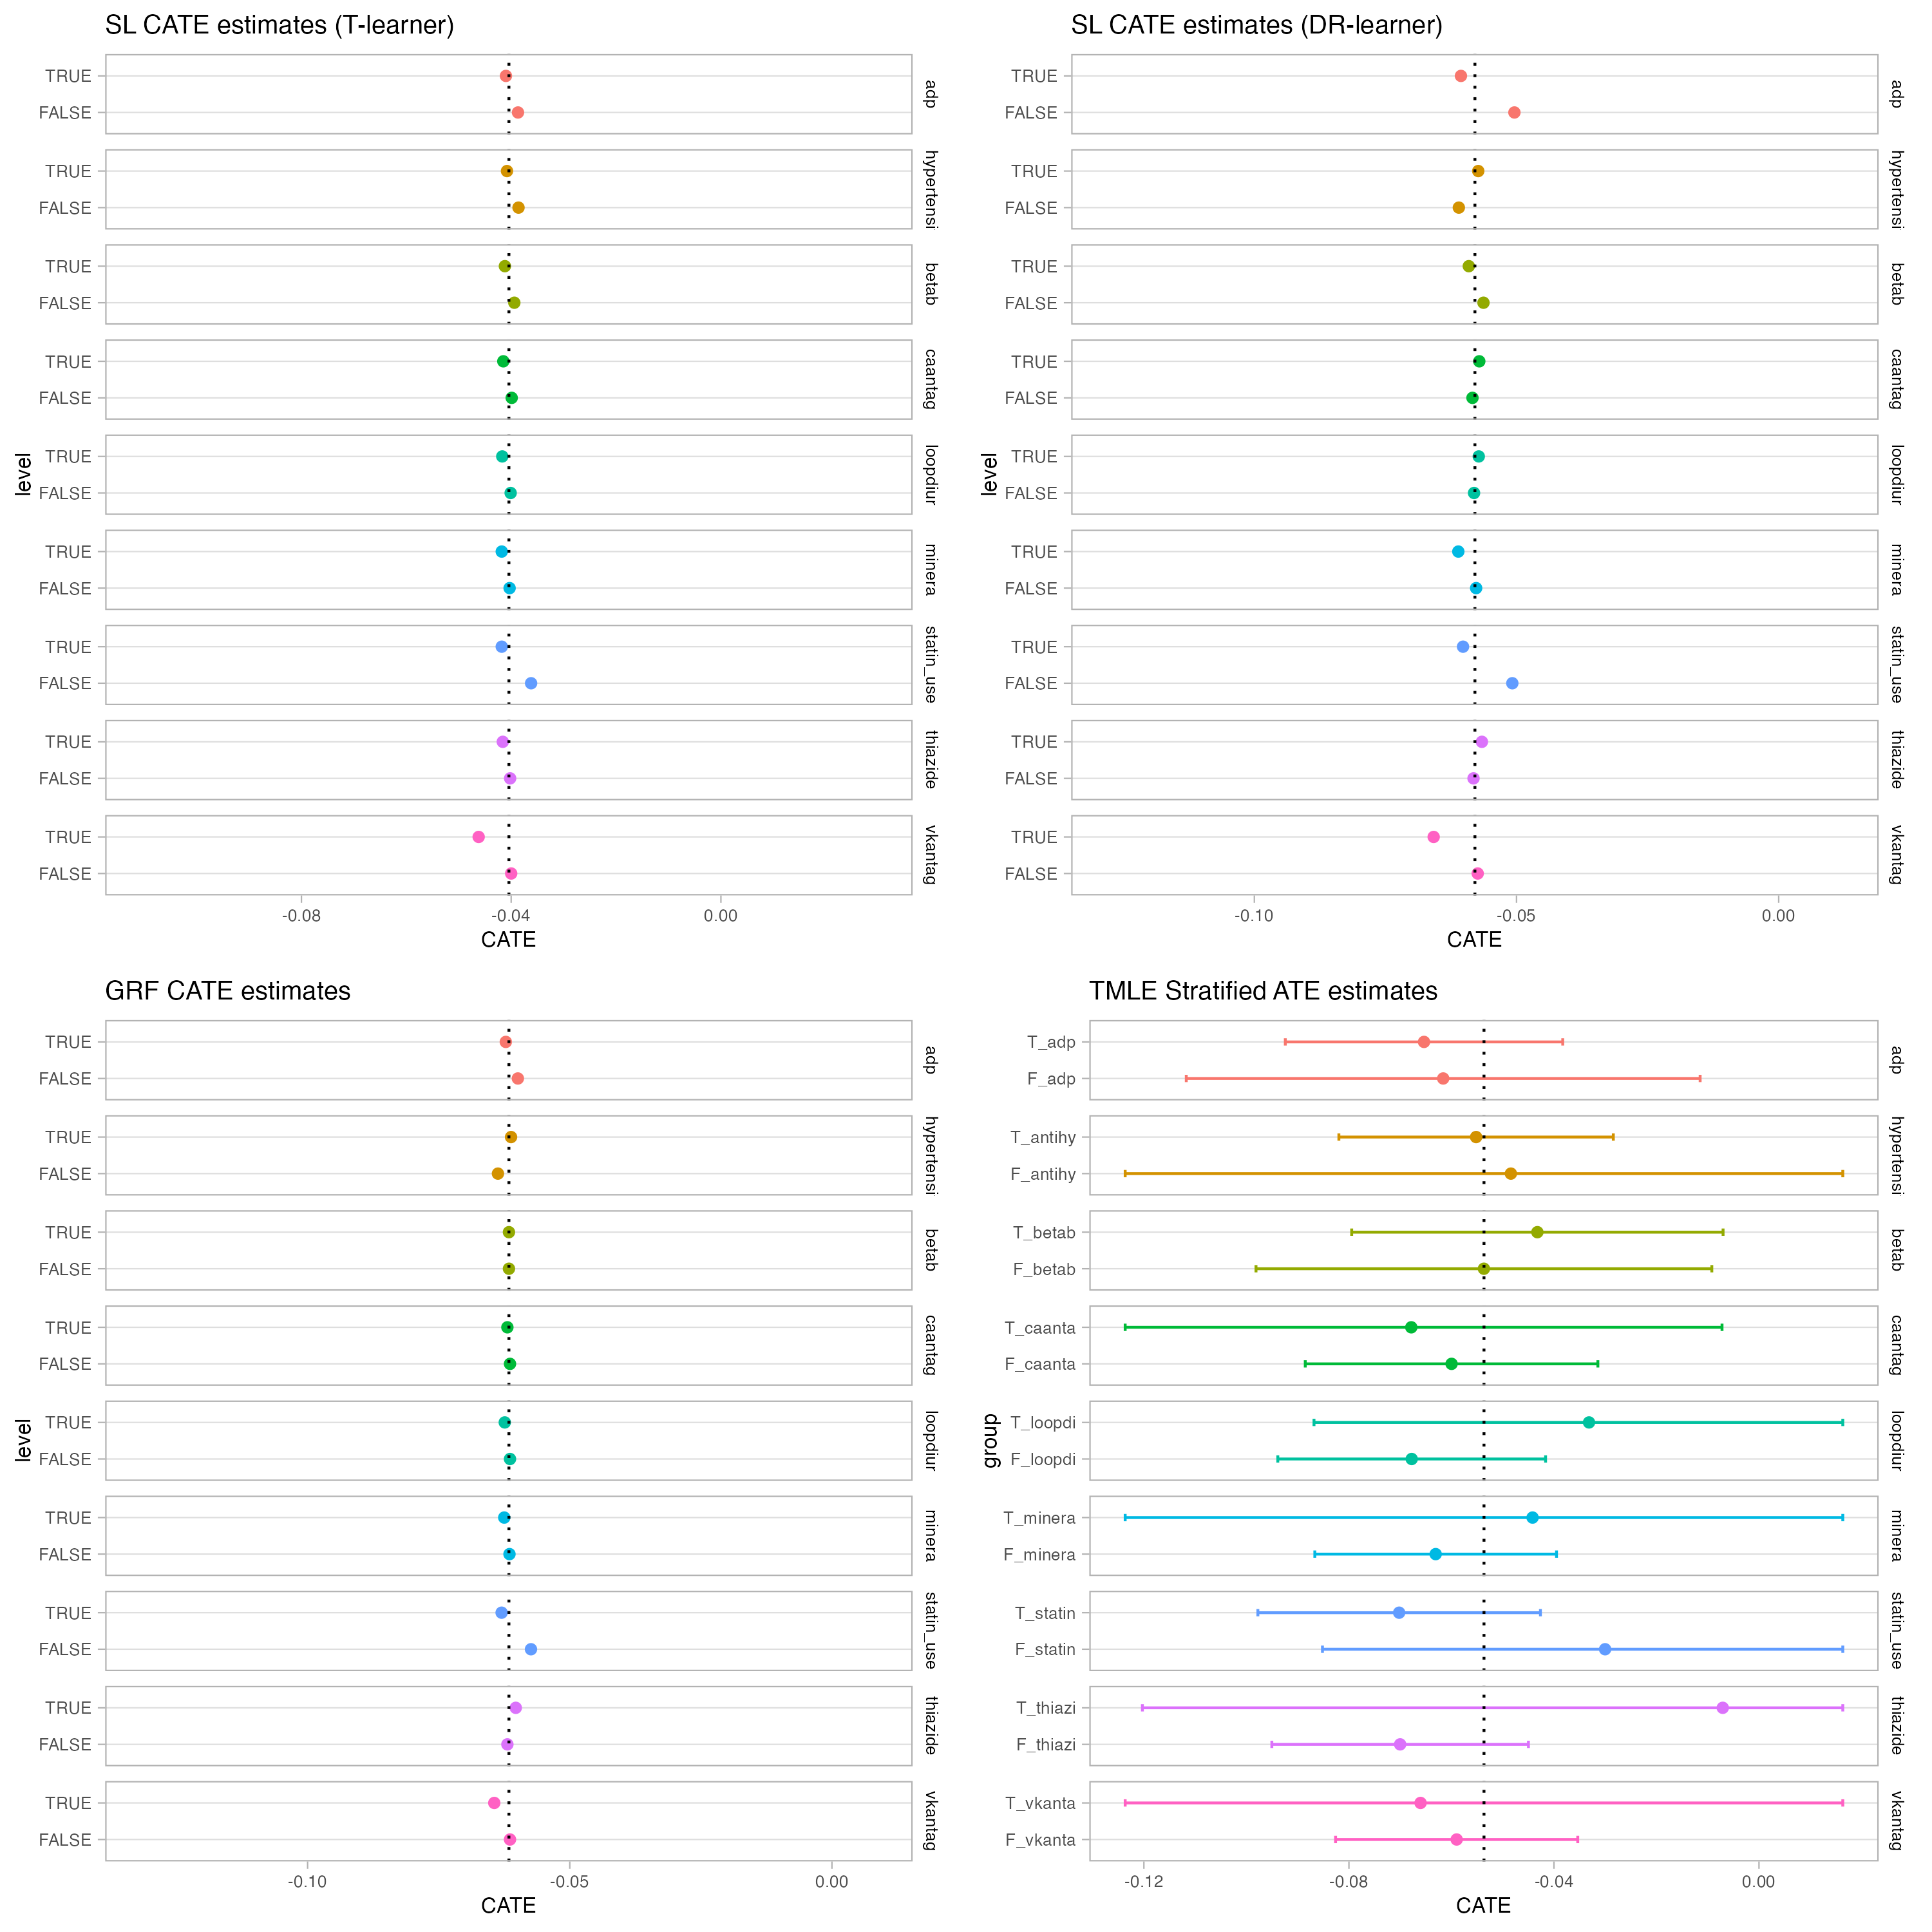
\includegraphics[width=1\linewidth]{plot/p_cate_all} 

}

\caption{CATE estiamtes}\label{fig:unnamed-chunk-10}
\end{figure}

\hypertarget{vte-estimation}{%
\subsection{4. VTE estimation}\label{vte-estimation}}

\begin{Shaded}
\begin{Highlighting}[]
\CommentTok{\# VTE }
\CommentTok{\# df\_fit$tau \textless{}{-} df\_fit$mu1\_hat {-} df\_fit$mu0\_hat}
\NormalTok{aipw\_vte }\OtherTok{\textless{}{-}} \FunctionTok{VTE}\NormalTok{(df\_fit, }\AttributeTok{method=}\StringTok{"AIPW"}\NormalTok{)}
\NormalTok{tmle\_vte }\OtherTok{\textless{}{-}} \FunctionTok{VTE}\NormalTok{(df\_fit, }\AttributeTok{method=}\StringTok{"TMLE"}\NormalTok{)}
\end{Highlighting}
\end{Shaded}

\begin{Shaded}
\begin{Highlighting}[]
\NormalTok{aipw\_vte}
\end{Highlighting}
\end{Shaded}

\begin{verbatim}
## 
## Call:
## VTE(data = df_fit, method = "AIPW")
## 
## Estimator: AIPW
## Estimate Values:
##            Estimate   Std.Error     CI_L        CI_U Wald.value  Wald.pval    
## ATE     -0.06141248  0.01087298 -0.08272 -0.04010144    31.9019 1.6216e-08 ***
## rootVTE  0.20028062  0.01158241  0.17758  0.22298215   299.0060 < 2.22e-16 ***
## VTE      0.04011233  0.00231973  0.03557  0.04465900   299.0060 < 2.22e-16 ***
## ---
## Signif. codes:  0 '***' 0.001 '**' 0.01 '*' 0.05 '.' 0.1 ' ' 1
\end{verbatim}

\begin{Shaded}
\begin{Highlighting}[]
\NormalTok{tmle\_vte}
\end{Highlighting}
\end{Shaded}

\begin{verbatim}
## 
## Call:
## VTE(data = df_fit, method = "TMLE")
## 
## Estimator: TMLE
## Estimate Values:
##            Estimate   Std.Error     CI_L        CI_U Wald.value  Wald.pval    
## ATE     -0.06021730  0.01083373 -0.08145 -0.03898319    30.8949 2.7239e-08 ***
## rootVTE  0.12140251  0.02729289  0.06791  0.17489657    19.7859 8.6618e-06 ***
## VTE      0.01473857  0.00331343  0.00824  0.02123288    19.7859 8.6618e-06 ***
## ---
## Signif. codes:  0 '***' 0.001 '**' 0.01 '*' 0.05 '.' 0.1 ' ' 1
\end{verbatim}

\hypertarget{vim-estimation}{%
\subsection{5. VIM estimation}\label{vim-estimation}}

\begin{figure}[H]

{\centering 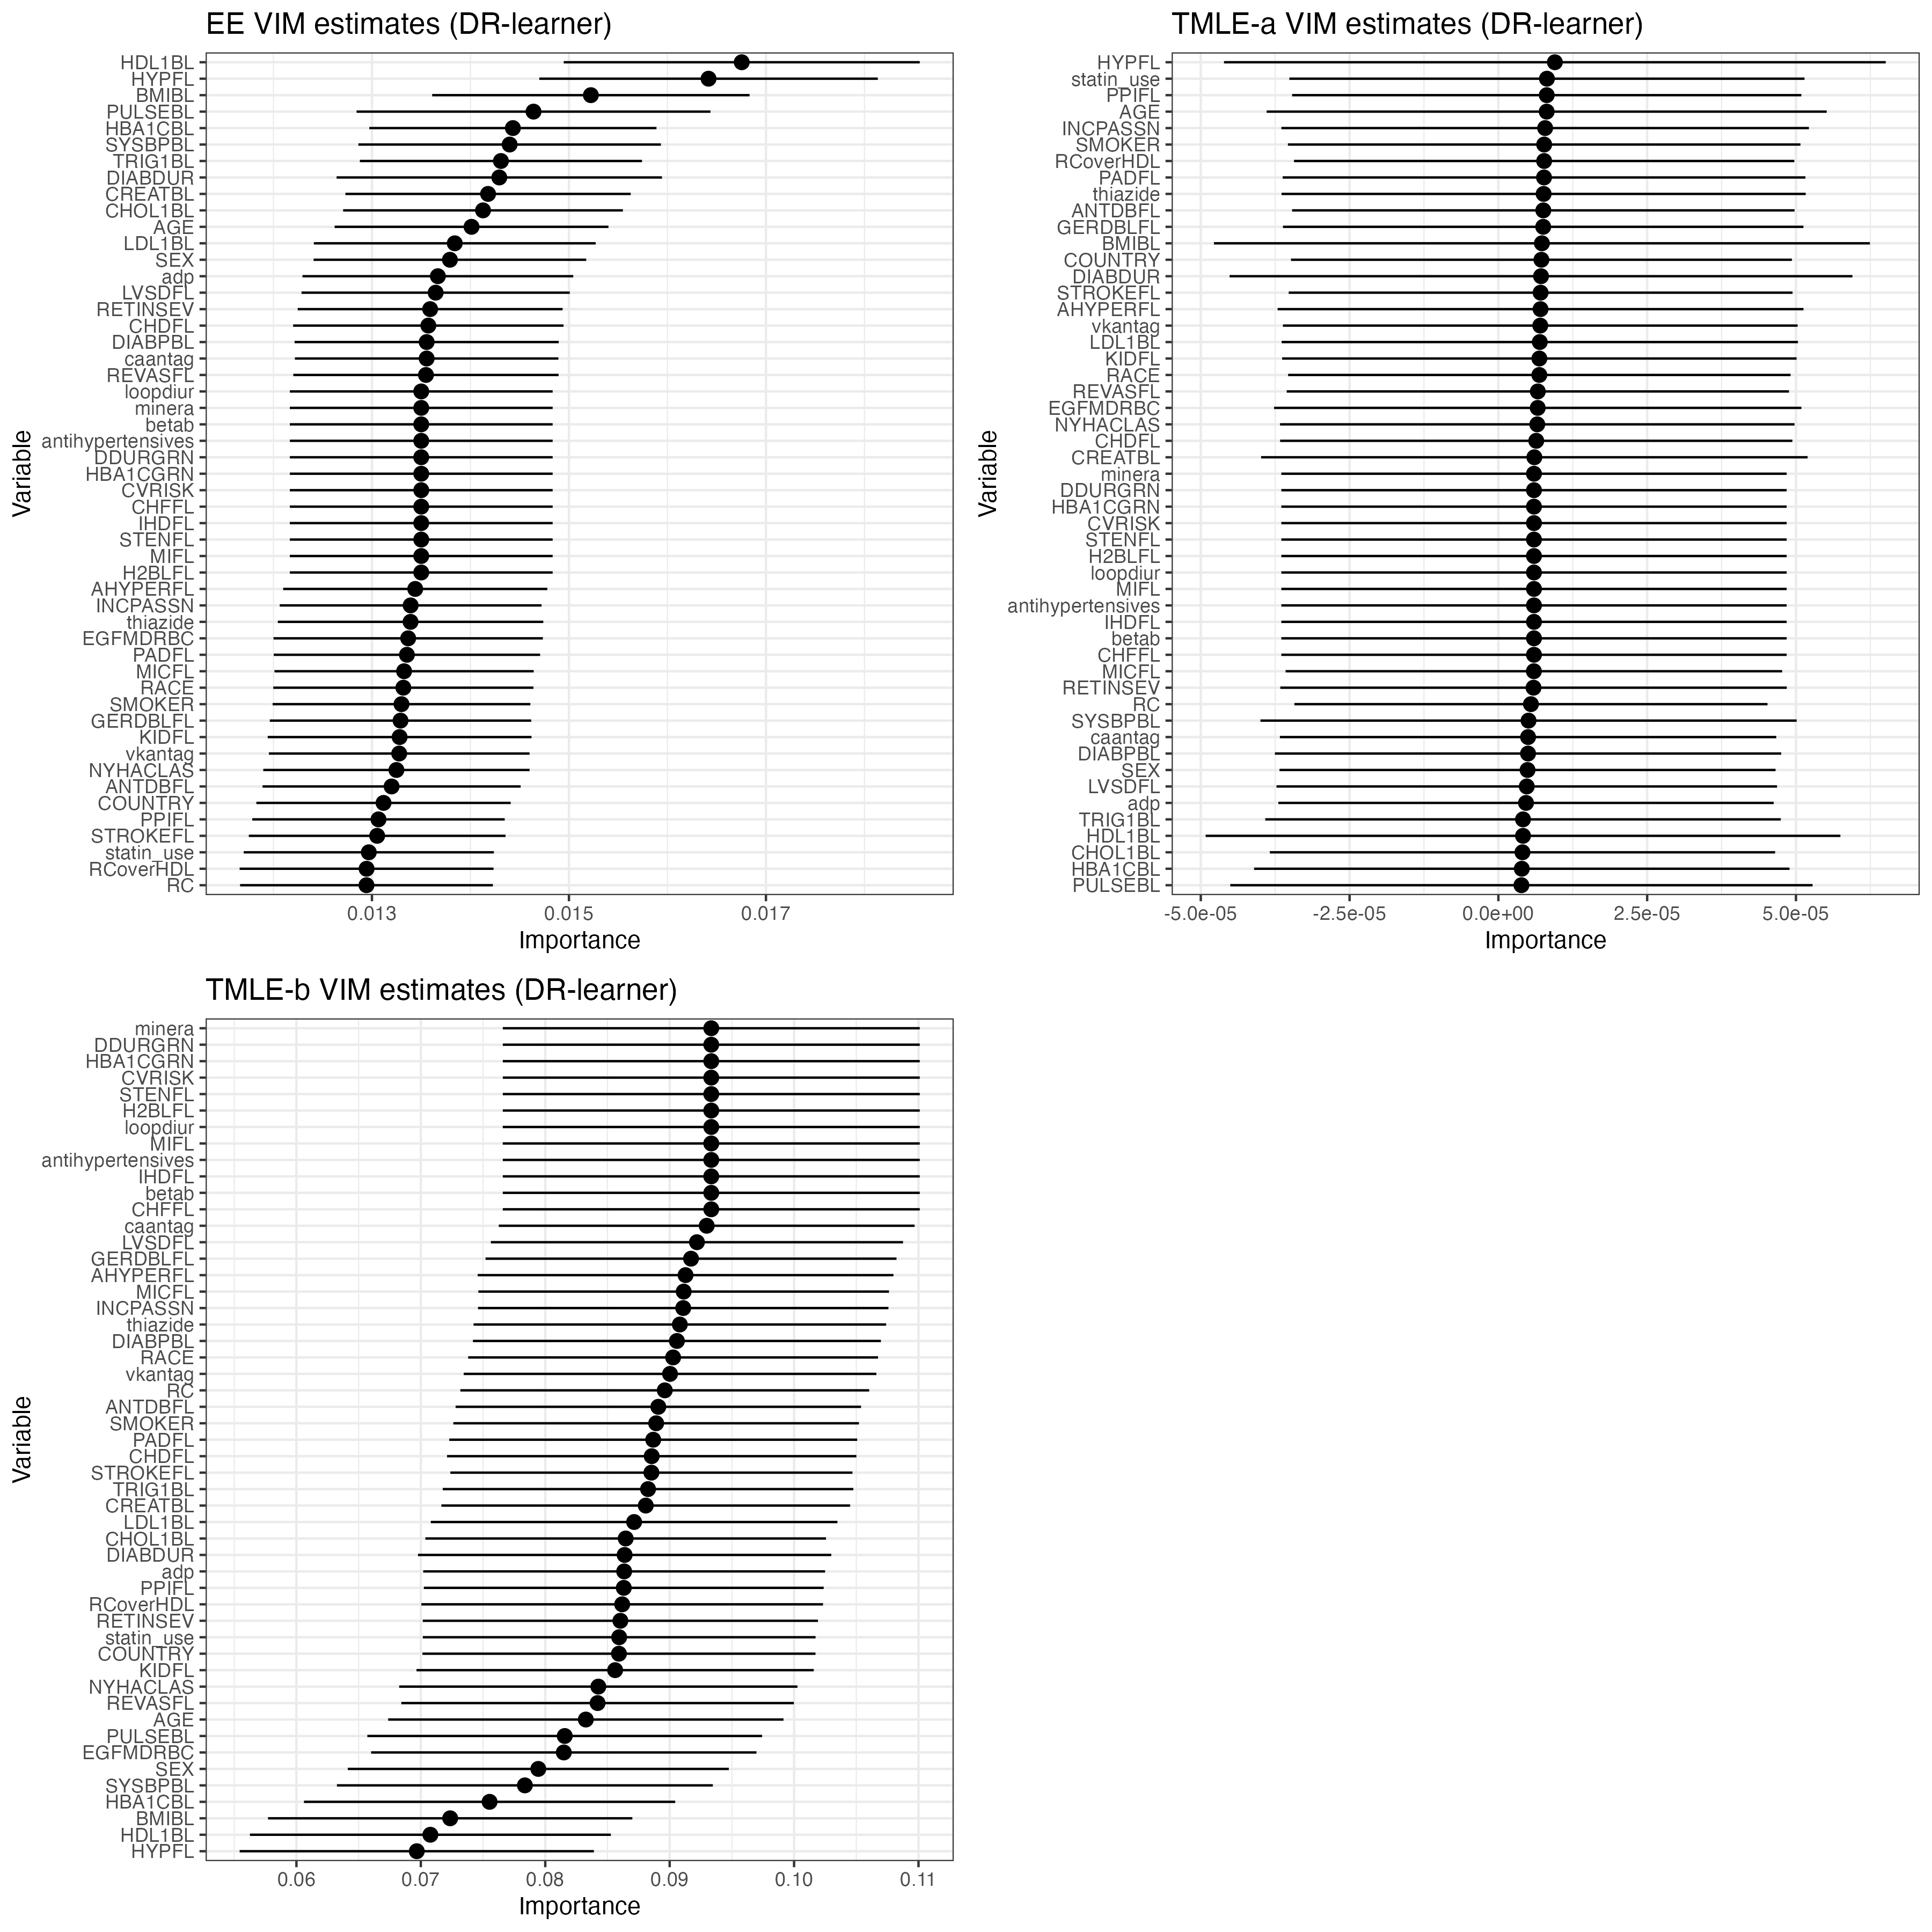
\includegraphics[width=1\linewidth]{plot/p_theta_all} 

}

\caption{VIM estiamtes}\label{fig:unnamed-chunk-17}
\end{figure}

\end{document}
